\section{Zephyr Project}


\subsection{Introduction}
Since Thread is a protocol for low-power, energy-efficient devices and its target market is smart homes, it is important to design devices that can meet the former criterion while maintaining high computing power. Modern microcontrollers with ARM Cortex-M cores are produced by a number of manufacturers with different peripherals, sometimes with very low power consumption. There are also solutions that integrate a radio module on-chip. These manufacturers, such as Nordic, Silicon Labs or STM, produce various free SDKs to facilitate the programming of their controllers. For the protocol uses the IEEE 802.15.4 standard. Nordic Semiconductors provides a separate SDK to support Thread access. However, in many cases, learning a new SDK is a dead time for a company, not to mention that if a company is designing universal devices using only some of the capabilities offered by the devices, they will have to modify their code for each device. Zephyr offers a solution to these problems.


\subsection{Zephyr Project}
The Zephyr Project is often referred to as a real-time operating system that targets processors with microcontrollers and other architectures used in embedded systems, but its architecture is much more complex, because in reality the operating system is only a small layer of the whole. It is essentially an open source project, associated with the Linux Foundation and designed to be implemented in safety-critical systems. 
The Zephyr OS can be broken down into three main parts
\begin{itemize}
    \item Kernel --- memory management, interrupt management, timing management etc.,
    \item Operating System Services --- peripheral management, hardware module management, error handling, etc.,
    \item Application Services --- management of paired devices (e.g.: Sensors), management of Internet protocols (e.g.: CoAP).
\end{itemize}


\subsection{Zephyr RTOS properties}
The \textit{Zephyr Real-Time-Operating-System}, or \textbf{RTOS}, has the following features
\begin{itemize}
    \item multithreading,
    \item interrupt handling,
    \item memory management,
    \item inter-thread messaging (between Zephyr OS Tasks),
    \item power management,
    \item memory protection (e.g.: overflow protection).
\end{itemize}

\subsection{The purpose of the Zephyr Project}
One of its main features, besides RTOS, is that it is very easy to compile the written source code to several kinds of devices without modifying the source code, only the settings. Another important feature is that there are third-party libraries implemented in the Zephyr project, so they are easy to use (such as OpenThread).

\begin{figure}[!htb]
    \centering
    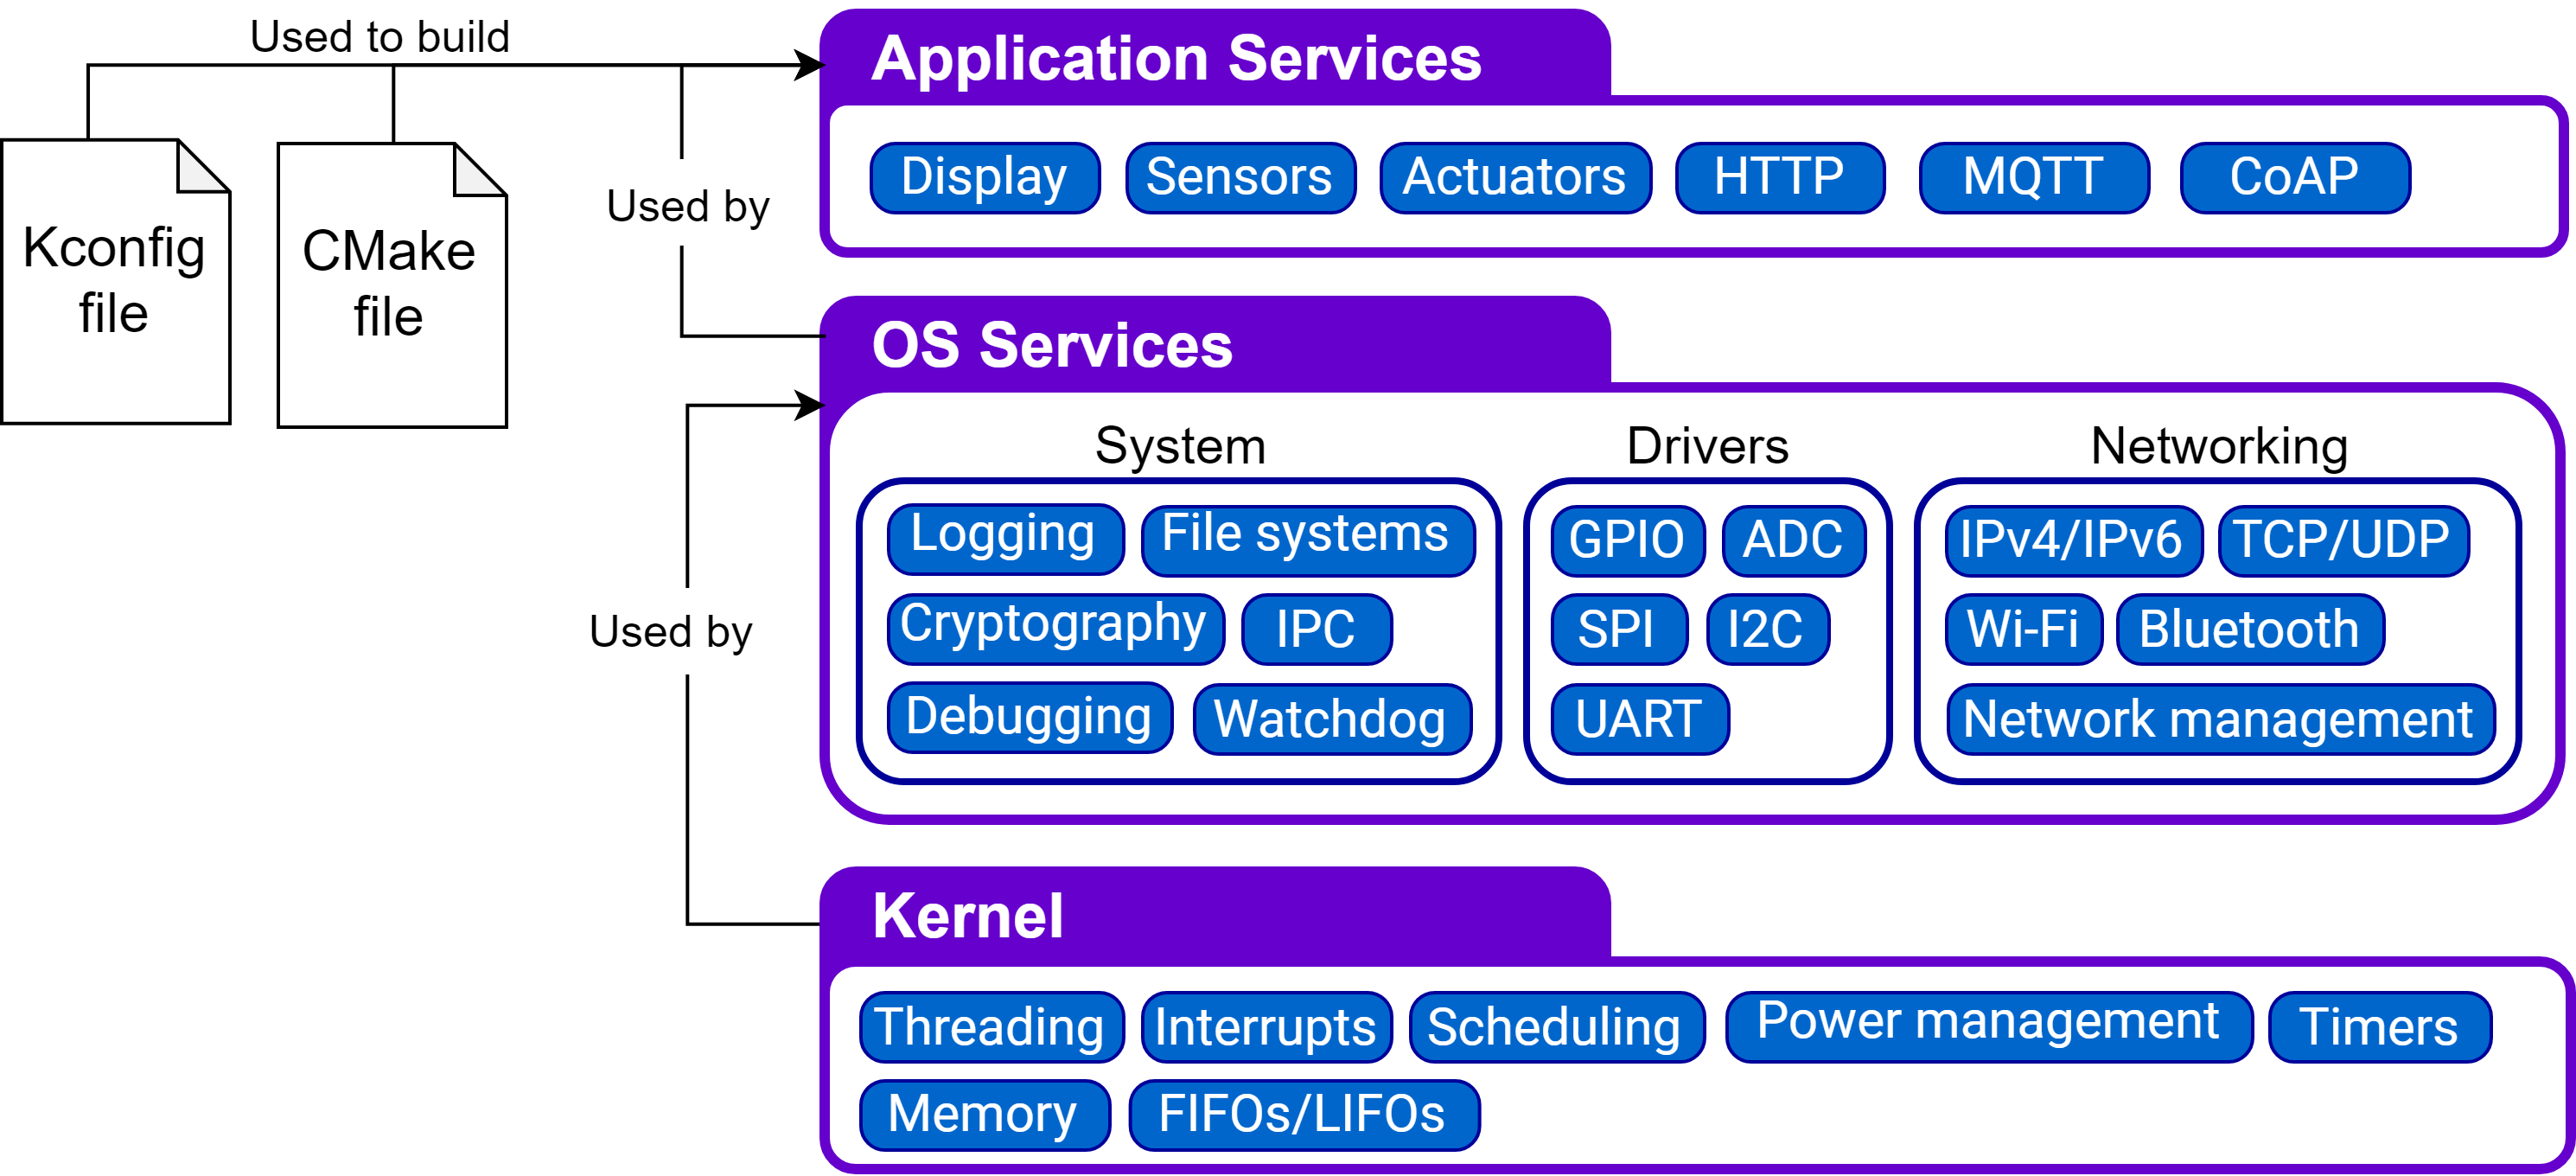
\includegraphics[scale=0.13]{img/Module_organization.png}
    \caption{Zephyr Project structure}
    \label{fig:Zephyrl}
    \cite{Zephyr}
\end{figure}


\subsection{Zephyr Project - Other programmes}

\subsubsection{DeviceTree}
It is also important to note that the Zephyr Project is cross-platform, i.e. available on Linux, MacOS and Windows operating systems. Zephyr uses \textbf{DeviceTree} to describe the hardware and for hardware portability. Essentially, in the configuration file of this program, certain functions can be named (such as LED1 or BUTTON0) or the address can be described of a particular register (such as I2C). This is advantageous because if the developer want to port a program to other hardware, only need to modify the DeviceTree description file (mostly files with .dts). For example, on an STM32F4 microcontroller, if there is a button placed, named BUTTON0 on GPIO24 and then do the same on an nRF52 for P0.31, the developer does not have to modify the code by mapping the different HAL libraries to each other, because Zephyr will do that for the developer. The hardware in this document was designed with a Nordic nRF52840 chip. Nordic Semiconductor has made two official releases of hardware with this chip, one is a development board called Development Kit (nRF52840DK) and the other is a Dongle, which can act like a module. The official use of this chip is to make a radio transceiver over an USB connection with the nRF Connect application. The dts description files for both hardware can be found pre-written in Zephyr, so by rewriting 1 line the whole source code was able to compiled from the Development Card to the Dongle, before the hardware design process.

\subsubsection{KConfig and CMake}
For software portability of the code, Zephyr uses \textbf{KConfig} to compile the used modules and drivers into the executable code at compile time. This program also helps to enable services and kernel modules when compiling the Linux kernel. The development also requires \textbf{CMake}, which adds the header and source files of the libraries to the project based on the path.

\subsubsection{Comparison of DeviceTree and KConfig}
In summary, the DeviceTree program does the hardware description, enables or disables hardware elements, enables interrupts and also sets the clock, from which it will set the microcontroller or processor at boot time. KConfig, on the other hand, will compile drivers and other libraries into Zephyr at compile time. Here is an an example of this for the better understanding. There are two applications in the same hardware environment with a controller, in which an I2C and a UART peripheral integrated. On the hardware there is an LED that is connected to a specific GPIO pin. One application the data is read from an I2C BME280 sensor and in the other case a LED is blinked. Since the same hardware must be used, the same DeviceTree descriptor structure is enough. From a software point of view, the I2C driver in the first application is needed, so KConfig should indicate this. Since the program only the I2C driver uses, KConfig will not include the other drivers at compile time, so the UART driver will not be included in the final code. In the second program, the same will happen, but the program code will not include the I2C driver.

\clearpage
\subsubsection{Example of the DeviceTree file structure}
\begin{lstlisting}
{
        compatible = "nordic,nrf-timer";
	status = "okay";
	reg = < 0x40009000 0x1000 >;
	cc-num = < 0x4 >;
	interrupts = < 0x9 0x1 >;
	prescaler = < 0x0 >;
	label = "TIMER_1";
};
\end{lstlisting}
\noindent
In this snippet of the DeviceTree file above, a timer is defined. This is an nRF timer built into a Nordic chip, which is enabled in the system (status="okay";). The address of the register block can be seen where this timer is located and how much space is reserved for this timer. The number of CC registers is 4. These are comparison registers whose function is to give an interrupt when the timer counter reaches the number stored in this registers. The interrupt is defined separately in the file what these values mean. And the penultimate line shows that this timer has no prescale. Furthermore, this timer will be referred in Zephyr as TIMER\_1. In this Nordic chip's documentation, it is able to find that the timer and actually has this register value associated with it. These .dts files own default values can be overwritten with an *.ovarlay file in the workspace directory of the program (or in some cases to the "boards" folder), where can be set the desired value by reference (for example by the status keyword, when the developer set "okay" to "disabled" and then this unit will be disabled).
\newline

\subsection{Nordic nRF52840}
The nRF52840 is a Nordic Semiconductors microcontroller, released in late 2017, designed for the 2.4\,\si{\giga\hertz} wireless market. The company provides a complete software SDK for Thread, Zigbee, Bluetooth LE (Low Energy) and Bluetooth Mesh networks. The code is executed by an ARM Cortex M4 core with a floating-point operation execution unit. It has 1\,\si{\mega B} of flash and 256\,\si{\kilo B} of RAM, which is only 30\% of the RAM and flash memory occupied by the complex OpenThread code of the Zephyr. It also has an internal DC/DC converter and an LDO so that it can be powered from its external USB power supply. Power is provided for external components through using DC/DC converter and LDO together. The maximum load current of the voltage converter's output is 25\,\si{\milli\ampere} according to the datasheet. The output voltage can be adjusted between 1.8\,\si{\volt} and 3.3\,\si{\volt} by setting two dedicated registers. It features ARM CryptoCell technology, which reduces the time needed to perform various encryptions. The IC also includes a number of communication peripherals such as USB\,2.0, QSPI, 32\,\si{\mega\hertz} SPI and several other timers and ADC modules. A full list of these functions are available on the second page of \href{https://infocenter.nordicsemi.com/pdf/nRF52840_PS_v1.1.pdf}{data sheet}\cite{NRFDATASHEET}.

\subsection{Summary of the Zephyr Project}
In this section I introduced the base functionalities of the Zephyr Project. More at the Zephyr RTOS and the essentially programs, which helps to the Zephyr's applications portability. I also presented the use case of DeviceTree in Zephyr and the differences between KConfig and DeviceTree programs. Finally, this section introduced the microcontroller, which I am using in this thesis. 